%!TEX root = ../Report.tex
%************************************************

% Algorithms

\chapter{Introduction}
The system operates on MIDI files. MIDI events are processed and the resulting notes are stored in a sequence where the pitch and duration of each note are recorded. A note is represented in MIDI as a number from $0$ to $127$.
Thus for each MIDI track a monophonic melody can be extracted.

A large set of MIDI files (~600) were collected for style of music. The following categories were used:
\begin{enumerate}
\item A mixture of Classical music (665)
\item A mixture of retro video game music (395)
\item A mixture of Pop and Top40 (1370)
\item A mixture of Classic Rock (2274)
\item A mixture of Jazz music (114)
\item A mixture of Dance and Techno (214)
\end{enumerate}

These categories are not the final list of styles that will be included into the end user application.


\chapter{Representation}
This section discusses how music is represented internally in the system and how the data structures are designed. 
Proper data structures are extremely important for good algorithms \footnote{Bad programmers worry about the code. Good programmers worry about data structures and their relationships. Linus Torvalds}.

\section{Assumptions and simplifications}
For this system our model of music is simplified and we do not make provisions for chords. Melodies are monophonic and are simply a list of notes of their durations.

Furthermore, we assume all MIDI files that correspond to \textbf{Track type $1$}.

\section{Note}
A note is the most basic element. A note consists of:
\begin{enumerate}
\item Note duration - A whole note, half note, quarter note and so on.
\item Note pitch - A number representing the note pitch, in MIDI scale. $0 \leq P < 128, p \in \mathbb{Z}$
\end{enumerate}

From these properties the following can be derived:
\begin{enumerate}
\item Octave - Every twelve note pitches represent one octave
\item Chromatic tone - An integer from 0 to 11. Also corresponds to the name of the note for example C, C\#, G, A\#
\end{enumerate}
These properties are related to the Note pitch by:
\[P = 12o + p \]
where $o$ is the octave and $p$ is the chromatic tone

\section{Melody sequence}
A melody sequence is simply a list or sequence of notes:
\[\{N_1, N_2, \ldots, N_n\} \]
Where $N$ is a note.

Most algorithms operate only on the melody sequence and output a melody sequence. Some algorithms may optionally require information on the instrument in which the melody sequence is played.

\section{Track}
A track contains a sequence of melody sequences and is also described by an instrument in which the sequence are played.

\section{Composition}
A composition is a sequence of tracks which can be played in parallel. 
MIDI files are converted into compositions.

\begin{figure}
\centerline{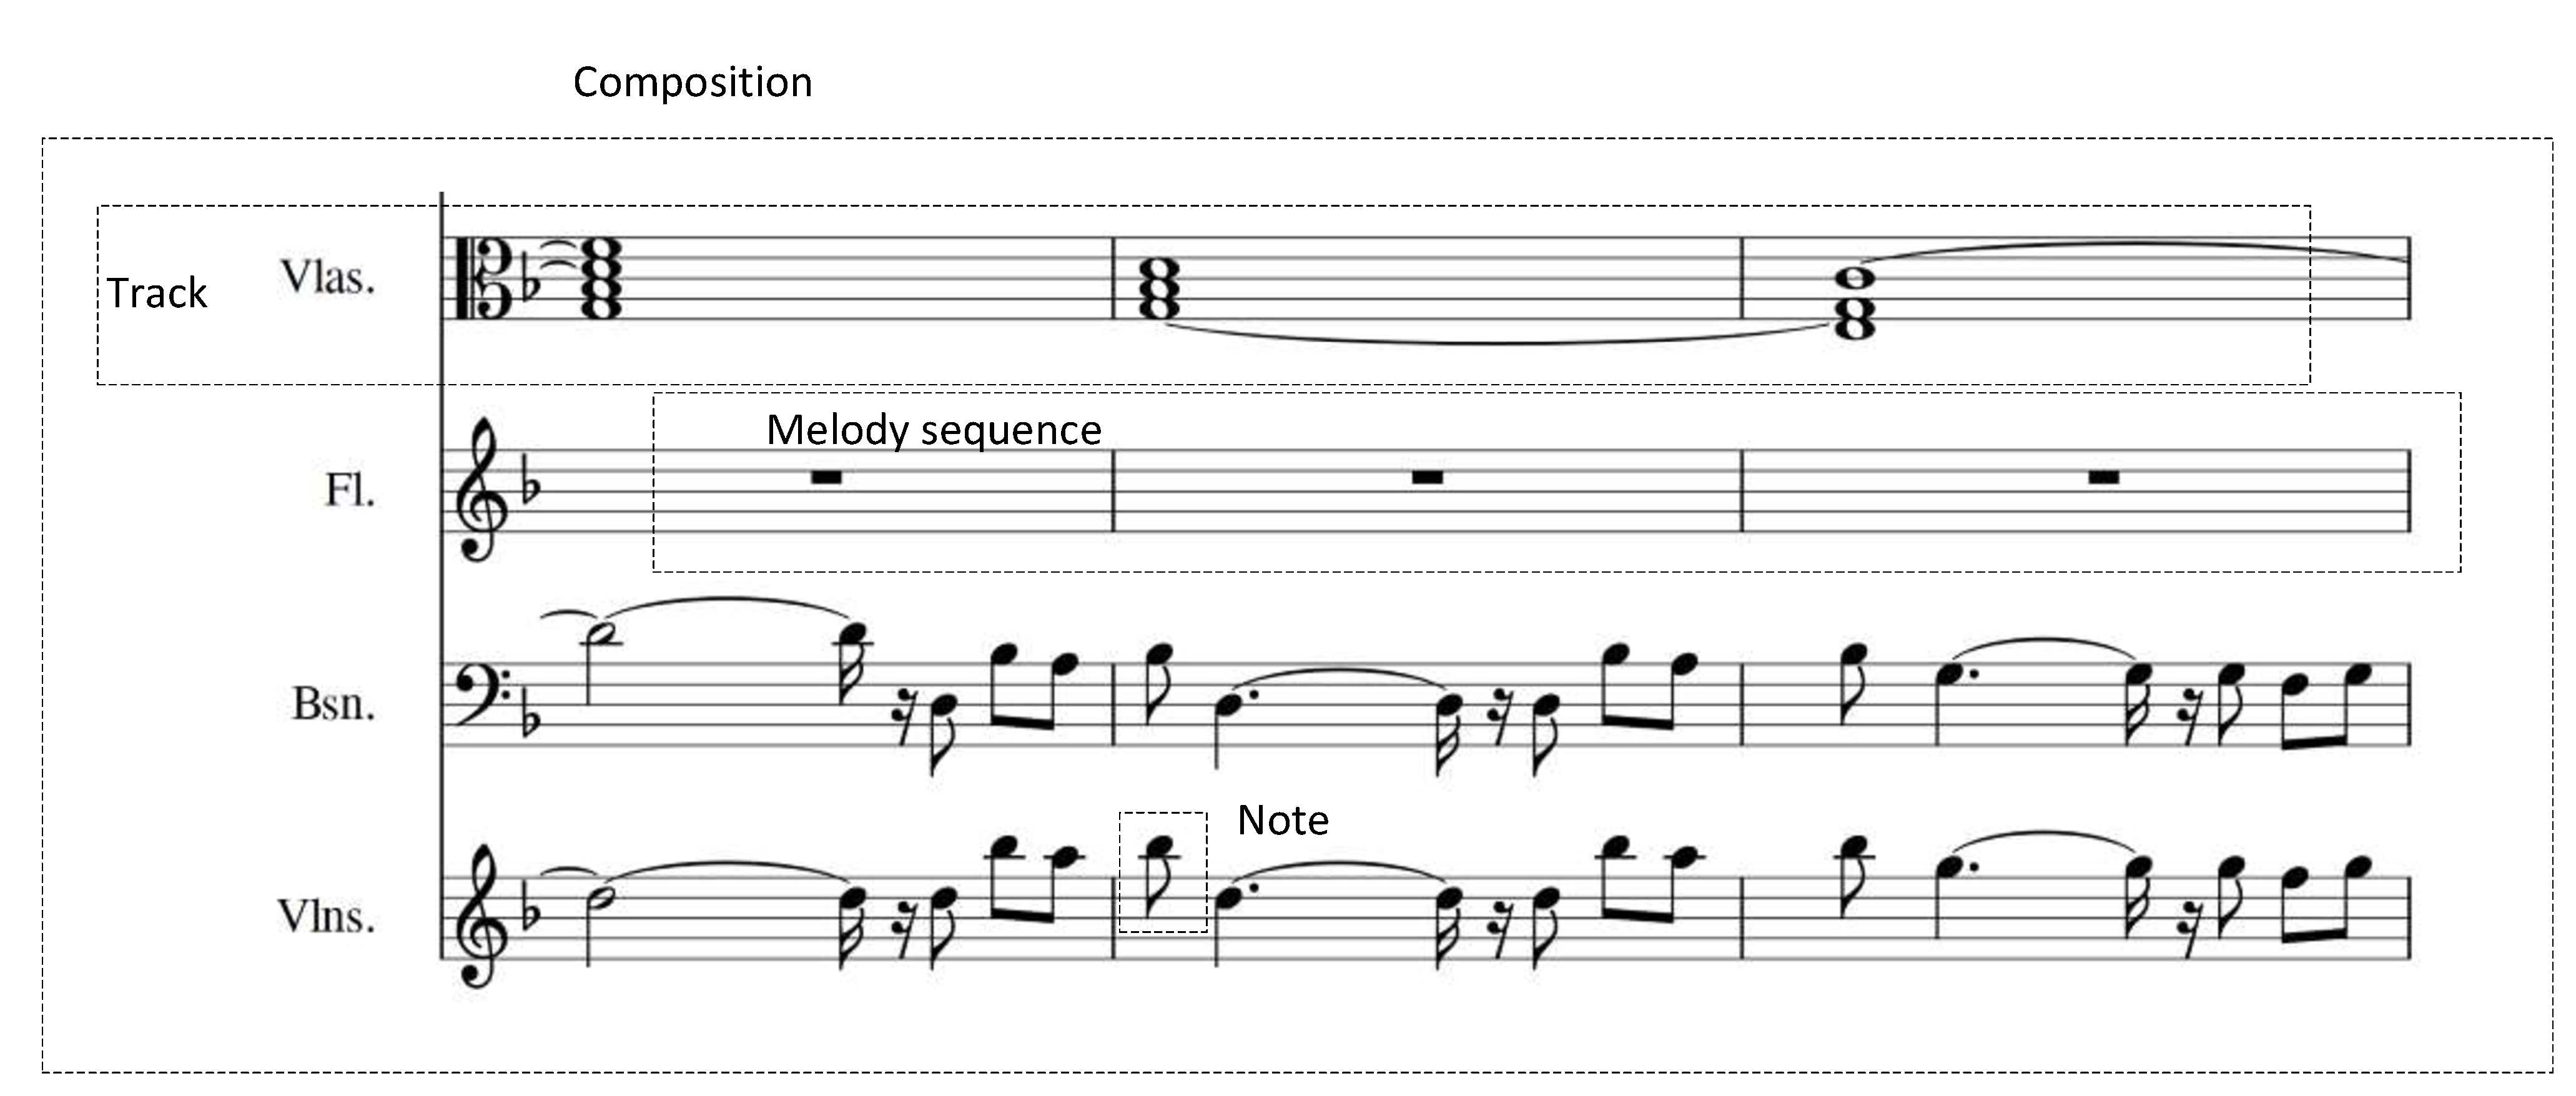
\includegraphics[width=400px]{../images/composition_illustration.pdf}}
\caption{Illustration of a composition and its elements}
\label{ims:compillu}
\end{figure}

Figure \ref{ims:compillu} illustrates the relation between the above mentioned structures for a midi file.

\begin{figure}
\centerline{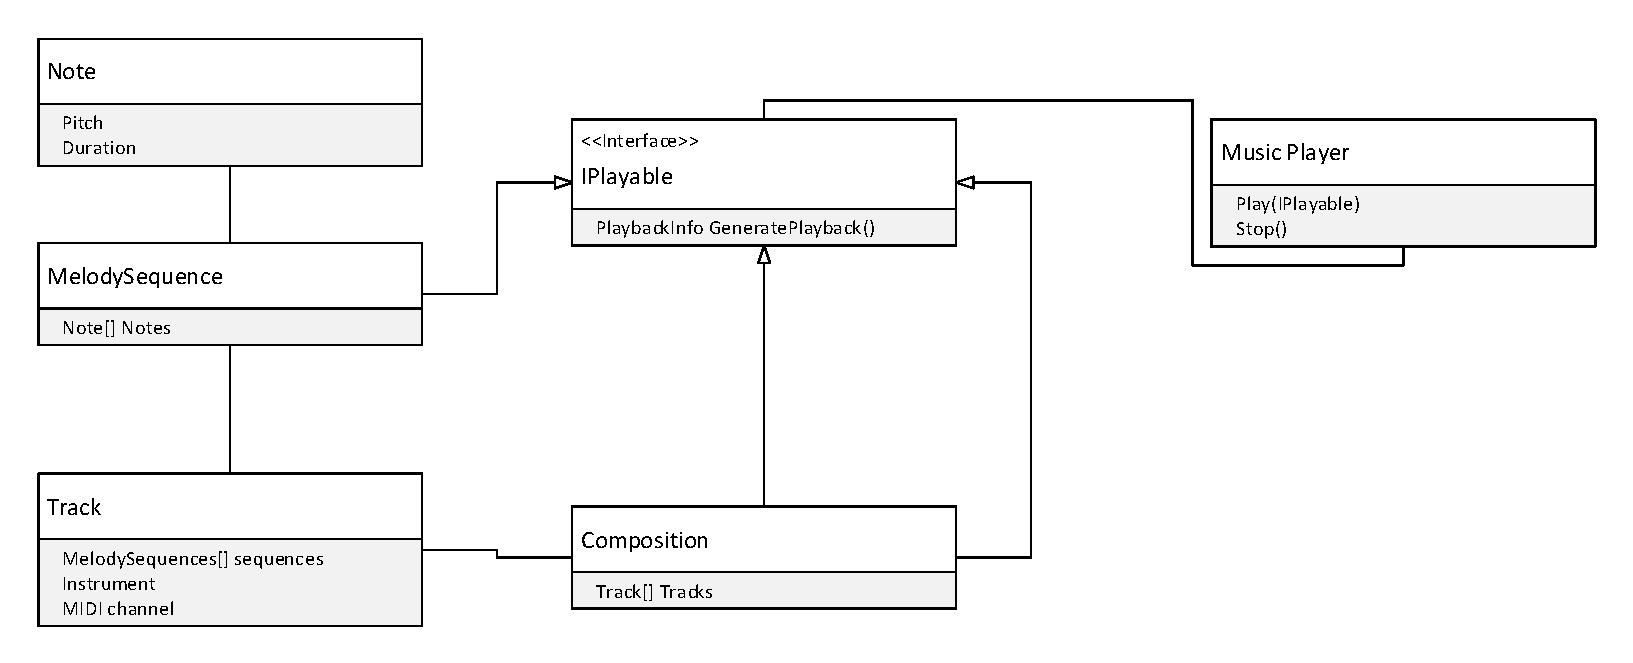
\includegraphics[width=400px]{../images/uml_notes.pdf}}
\caption{UML diagram indicating the interaction between composition elements}
\label{ims:uml_notes}
\end{figure}

Figure \ref{ims:uml_notes} indicates the interactions between Notes, Melody Sequences, Tracks, Compositions and the Music Player.

\section{Generator Algorithms}
In this section the data structures are discussed which aid with the generating of melody sequences through the algorithms that are discussed in this section. 
All algorithms considered in this section derive from the interface INoteGenerator. This exposes basic functionality for generating a algorithm and determining whether the Next function can be called. The Next function returns a new random melody sequence without resetting the generator. See figure \ref{ims:uml_generator}.

Using this abstracted design allows the user to select any algorithm to be used for composition, and the main application logic only needs to call Generate() or Next() as required.

\begin{figure}
\centerline{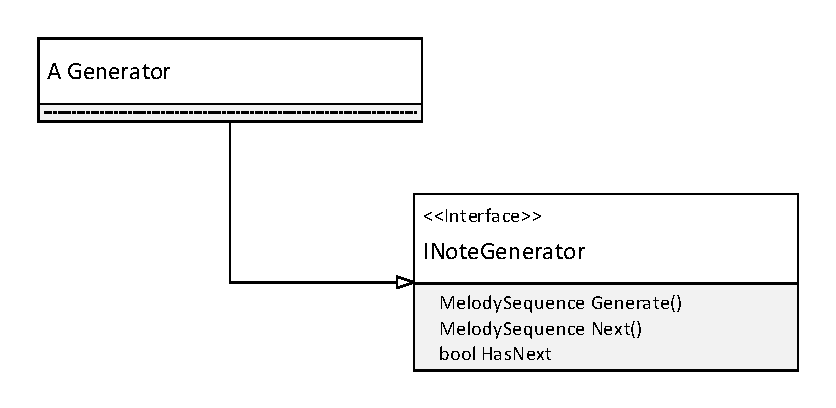
\includegraphics[width=250px]{../images/uml_generator.pdf}}
\caption{UML diagram of a generator class}
\label{ims:uml_generator}
\end{figure}

%%% START GENETIC %%%%%%%%%%%%%%%%%%%%%%%%%%%%%%%%%%%%%%%%%%%%%%%%%%%%%%%%%%%%%%%%%%%%%%%%%%%%%%%%%%%%%%%%%%%%%%%%%%%%%%%%%

%%%%%%%%%%%%%%%%%%%%%%%%%%%%%%%%%%%%%%%%%%%%%%%%%%%%%%%%%%%%%%%%%%%%%%%%%%%%%%%%%%%%%%%%%%%%%%%%%%%%%%%%%%%%%%%%%%%%%%%%%


\chapter{Genetic Algorithm for Melody Generation}

For this project a quantitative approach is taken toward algorithmic music composition. In particular quantitative metrics will be used in the fitness functions of the genetic algorithm.

In section \label{chap:comp_algo} the following types of music composition algorithms were investigated:
\begin{enumerate}
\item Neural Networks
\item Genetic Algorithms
\end{enumerate}
In the literature review, it was found that the pieces generated by neural networks lack musical coherency and perform poorly as the length of music increases. Some other attempts have met slightly more success although the overarching view for neural networks in music composition seems grim\footnote{Although neural networks as functions in genetic algorithms have had better success}.

The decision was made for genetic algorithms as the main composition algorithm for the following reasons:
\begin{enumerate}
\item They allow for great flexibility in implementation and music representation
\item The majority of research into machine learning music composition has been into genetic algorithm fitness functions
\item Great amount of variety made possible by different fitness functions and by the representation of music used in \acp{GA}
\end{enumerate}

Thus to reiterate, the algorithm employed in the application will be a \ac{GA}. As stated above a large amount of research has been into the fitness functions of different \acp{GA}.

In section \ref{sec:chapfitness} the following fitness functions were covered:
\begin{enumerate}
\item Zipf's law
\item Cosine similarity
\item Neural Networks
\item Normalized Compression Distance
\item Interactive evaluation\footnote{An interactive fitness function imposes a bottleneck on the performance of the system}
\end{enumerate}

\begin{figure}
\centerline{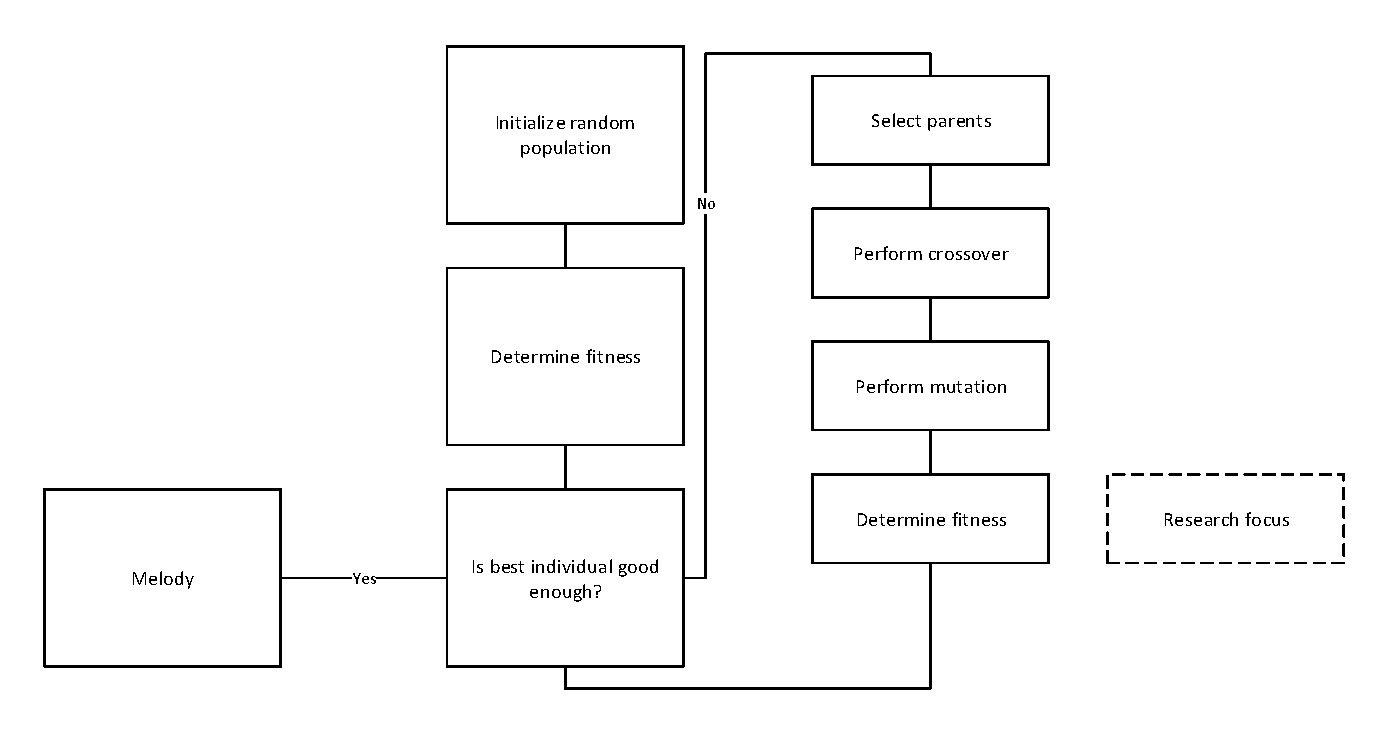
\includegraphics[width=400px]{../images/GA_flow.pdf}}
\caption{Flow diagram of the operation of a genetic algorithm}
\label{ims:geneticflow}
\end{figure}

Figure \ref{ims:geneticflow} indicates the flow for a genetic algorithm/program.

\section{Introduction}

Evolutionary algorithms come in a variety of different types. The two most common types found are Genetic Algorithms and Genetic Programming. Genetic Programming has been found to be more suitable for composing music than genetic programming due to music forming a hierarchical structure.

A flexible genetic programming model will be developed that is able to function with the investigated fitness functions. 

The two largest problems for a evolutionary computing problem is:
\begin{enumerate}
\item Obtaining a good representation of the problem
\item Obtaining a good fitness function
\end{enumerate}
A genetic algorithm modifies the structure of an individual, if the structure is poorly chosen then a optimal solution wont by found by the algorithm.
An ideal fitness function is able to quantify the fitness of an individual. An ideal fitness function in music composition would map the human perception of pleasantness into a fitness value. 

\section{Fitness functions}
The fitness function is a primary research interest in genetic music composition. An ideal fitness function captures the human perception of pleasantness in music.

Of the set of investigated fitness functions only the following functions will be implemented:
\begin{enumerate}
\item Cosine similarity
\item Neural networks
\item Normalized Compressions Distance
\end{enumerate}
Since interactive evaluation is slow and Zipf's law is superseded by Cosine similarity.

\section{Music Representation}
A flexible music representation will also be developed for the Genetic Programming algorithm. The representation will model \ac{MIDI} events and manipulation of them.
For example:
\begin{lstlisting}
  (d wn :=: f wn :=: a wn) :+:
  (g wn :=: b wn) :+:
  (c bn :=: e bn :=: g bn)
\end{lstlisting}
\begin{figure}
\center
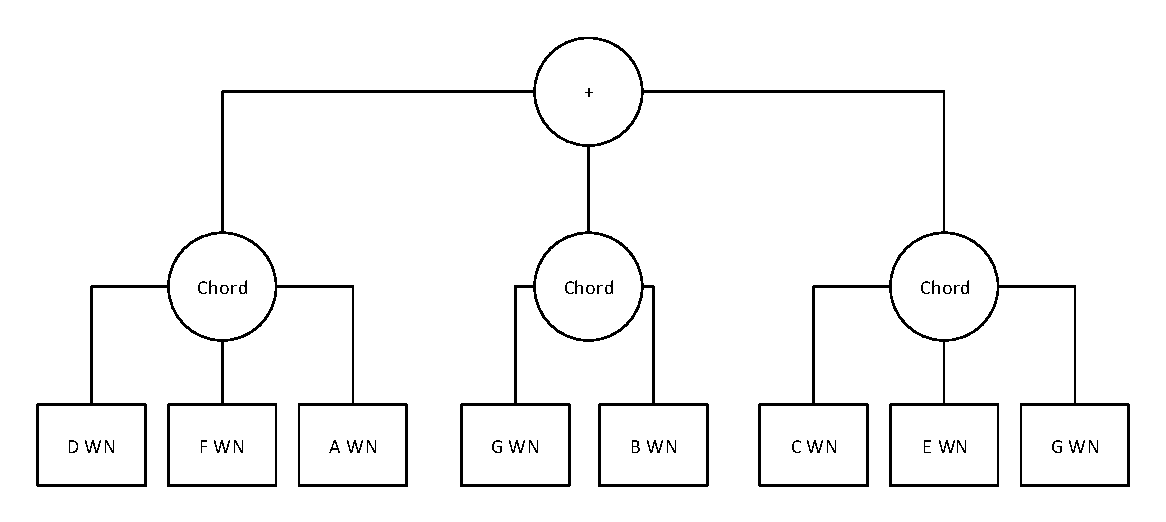
\includegraphics[width=400px]{../images/tree_stuct_piece.pdf}
\caption{A music piece in a tree structure}
\label{ims:musicpieceextrree}
\end{figure}
Where the :=: operator indicates pieces are played in parallel (chords) and :+: indicates pieces are played in series. a,b,d,e,f,g indicate the note pitch and wn indicates a whole note.
Figure \ref{ims:musicpieceextrree} indicates this in tree form. Strictly a chord is a set of three or more notes that are played simultaneously. Note that the second branch is only constituted of two notes.

Minsky and Laske \cite{Minsky1992} argued for a tree representation of music since the tree represents the hierarchical nature of music. The tree representation is much more complex than data structures such as vectors that are used in \acp{GA}.

Some authors \cite{Biles1994} limit the search space by ensuring that melodies are in a certain scale 

\section{Genetic operators}
Several different operators can be performed on the tree structure. In figure \ref{ims:musicpieceextrree} the serial concatenation and parallel concatenation operators were shown.
Some additional operators which may be employed include:
\begin{itemize}
\item Repetition - Repeating a segment a given number of times
\item Shift note pitches - Shift all pitches of notes by a certain amount
\item Duration elongation or contraction - For example a slow operation doubles the duration
\item Transposition - Moving note positions relatively
\item Retrograde - Reversed order of notes
\end{itemize}

Genetic operations such as mutation and crossover may be used conventionally.

\section{Metrics} \label{chap:metrics}
Feature extraction is required to reduce the search space and to provide the fitness function with musically meaningful measures with which to rate the fitness. In this section we cover some quantitative metrics that may be used as measures to identify or represent music.

The frequencies of a metric is used in the Cosine Similarity fitness function.

The different types of metrics that will be used include:
\begin{enumerate}
\item Pitch - List of pitches
\item Pitch differences - Store first pitch, thereafter list consecutive pitch differences
\item Chromatic tone - 12 pitch class. Notes are reorganized into 12 classes.
\item Note durations - durations of notes
\item Pitch distance - intervals between repetition of pitches
\item Chromatic tone distance - intervals between repetition of chromatic tones  
\item Melodic interval - intervals between the current note and the previous note
\item Melodic bi-gram - Pairs of melodic intervals
\item Rhythm - duration of a note in addition to the following rest
\item Rhythmic interval - relationship between adjacent note rhythms
\item Rhythmic bi-gram - Pairs of adjacent rhythmic intervals.
\item Chromatic tone duration - A pair of the chromatic tone and the duration
\end{enumerate}

Let $p$ denote the pitch of the note, where $0 \leq p < 128$.
Then the chromatic tone is given by:
\[c = p \% 12\]
where $\%$ indicates the modulo operation.
The melodic interval is given by:
\[\text{mi}_k = p_k - p_{k-1} \]
The melodic bi-gram is given by:
\[b_k = (\text{mi}_k, \text{mi}_{k+1}) \]
Let $r$ indicate the note duration with rests
Then the rhythmic interval is given by:
\[\text{}ri_k = \frac{r_k}{r_{k-1}} \]
and the rhythmic bi-gram
\[\text{rk}_k = (\text{ri}_k, \text{ri}_r) \]

In this manner we can build a metric vector, let $m_i(A)$ denote a metric's value at position $i$ for musical piece $A$. Then the metric vector is given by $\vec{M}_A = \{m_0(A), m_1(A), \ldots, m_n(A) \}$ 


\section{Fitness functions}

In this section two fitness functions are described which can be used for the Genetic Algorithm. \ac{NCD} and Cosine Similarity are described here.

The fitness functions described in this section require the phenotype of an individual. Thus it is necessary to parse the genotype, the genetic tree of the individual down into a sequence of notes.

\subsection{Cosine similarity}
Some fitness functions such as Cosine similarity and Zipf's law operate on the features of music. 

Cosine similarity can be applied to the metrics listed in section \ref{chap:metrics}. Let $\vec{M_A}$ denote the vector of metric values according to a metric $m$ for a music piece $A$ and $\vec{M_B}$ denote the vector by $m$ for a music piece $B$ then the similarity between $A$ and $B$ is given by:
\[\text{similarity}_m(A,B) = \frac{\vec{a} \cdot \vec{b}}{|\vec{a}| |\vec{b}|}\]

A set of metrics may be used. 
The fitness function is then given by a weighted average:
\[f = \frac{1}{N} \sum_{k}^N w_k \times \text{similarity}_{mk}(A,B) \]
where $w$ is a weight assigned to metric $mk$.

\subsection{Normalized compression distance}
In order to utilize \ac{NCD} both pieces being tested need to be encoded in the same way. Musical pieces may be encoded as metric vectors as listed in section \ref{chap:metrics}. More complex metrics may be utilized however there has been no thorough investigation into this.

The \ac{NCD} as an estimate to the \ac{NID} was covered in section \ref{sec:class_ncd}.

In order to utilize the \ac{NCD} as a fitness function the following steps are taken:
\begin{enumerate}
\item Encode a set from the \ac{MIDI} library according to a metric. Let $\Omega = \{\vec{M_0}, \vec{M_1}, \ldots, \vec{M_n}\}$ for musical pieces $0$ to $n$ in the \ac{MIDI} library that accord to a certain style.
\item Encode the population individual $x$ according to the metric (Given by $\vec{M_x}$).
\item Employ the fitness function
\end{enumerate}

The fitness function that will be used is:
\[f(x) =  \left(\sum_{\vec{T}\in\Omega} \text{NCD}(\vec{M_x}, \vec{T}) \right)^{-1}\]

\section{Methodology}
%TODO
In this section the setup and parameters of the experiment to produce melodies with Genetic Algorithms are outlined.

In order to compose a melody with a genetic algorithm a fitness function is required to rate the fitness of an individual. The following fitness functions were investigated:
\begin{enumerate}
\item \ac{NCD}
\item Cosine similarity
\end{enumerate}

A proper representation is required. A melody is represented in tree form. The tree is given a maximum depth of $(\log_2 x) +  3$ where $x$ is the average number of notes in a melody.

The following genetic operators were used:
\begin{enumerate}
\item Concatenation - The addition of two nodes
\item Duration Shift - Scale the duration with a factor
\item Pitch Shift - Move all note pitches a certain number up or down
\item Repeat - Repeat a note a certain number of times
\item Swap - Swap the positions of two notes
\end{enumerate}

The following metrics were investigated:
The different types of metrics that will be used include:
\begin{enumerate}
\item Pitch differences
\item Chromatic tone duration 
\item Chromatic tone distance 
\item Pitch distance
\item Melodic interval
\item Melodic bi-gram
\item Rhythmic interval 
\item Rhythmic bi-gram
\end{enumerate}

The duration and pitch a note may take on is limited to the available note pitches and durations in the dataset.

The parameters of the Genetic Algorithm were set as follows:
\begin{itemize}
\item Chromosome representation - Tree form
\item Mutation rate - 0.1
\item Crossover rate - 0.9
\item Population - 30
\item Selection - Elite selection
\item Auto shuffling of individuals in population after every epoch
\item Standard amount of generations - 1000
\end{itemize}

The individual with the highest fitness was used as the resulting chromosome. 
Since the result is in tree form it needs to be parsed into a simple sequence of notes.

\section{Results}


A simple test was done comparing the \ac{NCD} and Cosine Similarity fitness functions against each other. The Cosine Similarity was tested using the Chromatic Time Duration, Rhythmic Bigram and Melodic Bigram frequency metrics. The average fitness and maximum fitness were compared against each other. The genetic algorithm was run for $100$ epochs.

% Table generated by Excel2LaTeX from sheet 'Sheet3'
\begin{table}[htbp]
  \centering
  \caption{Comparison of Fitness Functions}
    \begin{tabular}{l|rr}
    \toprule
          & Performance &  \\
    \midrule
          & Average Fitness & Maximum Fitness \\
    NCD   & 0.0016 & 0.00156 \\
    Metric Similarity & 0.666 & 0.683 \\
    \bottomrule
    \end{tabular}%
  \label{tab:ffcompare}%
\end{table}%

Table \ref{tab:ffcompare} shows the results. It can be seen that the maximum fitness achieved by the \ac{NCD} fitness function in 100 epochs is only $0.0016$ whereas the MetricSimilarity is at $0.683$. The pleasantness of the produced melody by \ac{NCD} is also worse, however this may be due to the lower fitness.
However generation time is important for the Genetic Algorithm and the \ac{NCD} fitness function is slow.


% Table generated by Excel2LaTeX from sheet 'Sheet3'
\begin{table}[htbp]
  \centering
  \caption{Performance comparison between frequency metrics}
    \begin{tabular}{l|llll}
    \toprule
          & MaxFit & AvgFit & Time(ms) & Pleasantness \\
    \midrule
    Chromatic Tone & 0.944 & 0.9439 & 8992  & 4 \\
    Chromatic Tone Distance & 0.98  & 0.98  & 11017 & 5 \\
    Chromatic Tone Duration & 0.936 & 0.935 & 13688 & 5 \\
    Melodic Bigram & 0.857 & 0.857 & 3900  & 5 \\
    Melodic Interval & 0.985 & 0.985 & 9037  & 5 \\
    Pitch & 0.832 & 0.832 & 14001 & 4 \\
    Pitch Distance & -     & -     & -     & - \\
    Rhythm & 0.952 & 0.952 & 367   & 4 \\
    Rhythmic Bigram & 0.995 & 0.995 & 4729  & 7 \\
    Rhythmic Interval & 0.996 & 0.996 & 5501  & 6 \\
    \bottomrule
    \end{tabular}%
  \label{tab:metriccomp}%
\end{table}%

The maximum fitness, average fitness, time (given in milliseconds) and subjective pleasantness were evaluated for each frequency metric. See table \ref{tab:metriccomp}. 

In order to construct a target piece for the metric similarity the notes of the first track of each midi file were sequenced. The total notes were $662923$. Note that some metrics have larger time than others, this is due to the amount of features or categories for that metric and does not necessarily indicate that metric is slow. The pitch distance metric was excluded as it took too long.

From table \ref{tab:metriccomp} it can be seen that subjectively rhythm is important.




\begin{figure}
\centerline{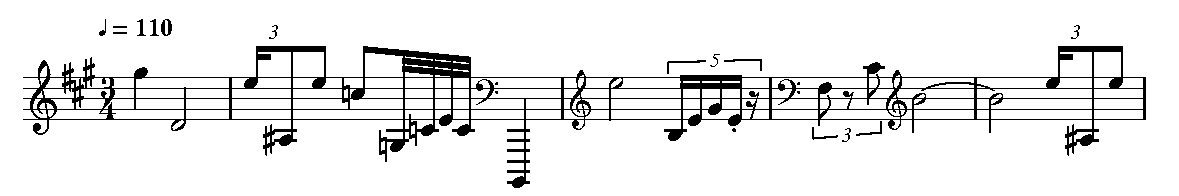
\includegraphics[width=300px]{../images/genetic_ncd.pdf}}
\caption{Melody produced with a Genetic Algorithm using the \ac{NCD} fitness function}
\label{ims:genetic_mel_ncd}
\end{figure}

\begin{figure}
\centerline{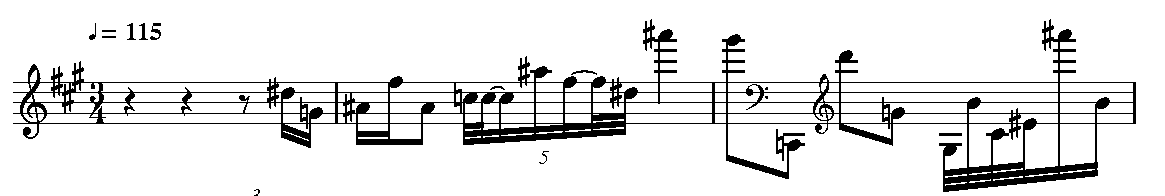
\includegraphics[width=300px]{../images/genetic_cosine_ctd_rb.pdf}}
\caption{Melody produced with a Genetic Algorithm using the cosine similarity fitness function with chromatic tone duration and rhythmic bigram metrics}
\label{ims:genetic_mel_ctdrb}
\end{figure}

\begin{figure}
\centerline{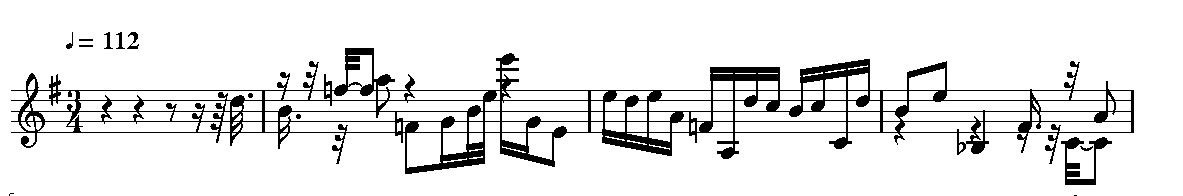
\includegraphics[width=300px]{../images/genetic_cosine_all.pdf}}
\caption{Melody produced with a Genetic Algorithm using the cosine similarity fitness function with all frequency metrics}
\label{ims:genetic_mel_mall}
\end{figure}

Figure \ref{ims:genetic_mel_ncd} indicates an excerpt of a melody produced with the Genetic Algorithm using the \ac{NCD} fitness function. The \ac{NCD} fitness function produced the worst results. The resulting melodies sounding chaotic and random. \ac{NCD} is also slow, as each individual needs to be converted to its text representation and then be compressed in order to obtain its compressed distance.

The melody produced in figure \ref{ims:genetic_mel_ctdrb} using the cosine similarity fitness function was rather pleasant and the rhythmic bigram and chromatic tone duration -frequency metrics produce pleasant melodies.

The melody produced in figure \ref{ims:genetic_mel_mall} used the cosine similarity fitness function using all the frequency metrics. At times the melody is pleasant however off-sounding or out of key notes are a common occurence. The melodies also dont have structure. This indicates that some of the frequency metrics either don't work well in conjunction with each other or some frequency metrics have a negative effect on the pleasantness of melodies. 

The following frequency metrics produced good or pleasant results:
\begin{enumerate}
\item Chromatic tone distance - intervals between repetition of chromatic tones
\item Melodic interval - intervals between the current note and the previous note
\item Rhythmic bigram - Pairs of adjacent rhythmic intervals
\item Chromatic tone duration - A pair of the chromatic tone and the duration
\end{enumerate}


\section{Conclusion}

The decision was made to utilize a genetic programming algorithm since the tree structure accommodates the hierarchical nature of music. Genetic programming provides flexibility, variety of possible styles and a large amount of research has been done one fitness functions for genetic algorithms.

Fitness functions require good measures that make it possible to rate musical pieces quantitatively. A set of metrics were developed in which musical pieces can be measured.

Two fitness functions, namely Cosine similarity and \ac{NCD} were developed to incorporate these metrics.

The results of different fitness functions were compared. \ac{NCD} performed the worst. Not all of the frequency metrics required for the cosine similarity fitness function produced good results. A subset of good frequency metrics were explored.


%%% END GENETIC %%%%%%%%%%%%%%%%%%%%%%%%%%%%%%%%%%%%%%%%%%%%%%%%%%%%%%%%%%%%%%%%%%%%%%%%%%%%%%%%%%%%%%%%%%%%%%%%%%%%%%%%%

%%%%%%%%%%%%%%%%%%%%%%%%%%%%%%%%%%%%%%%%%%%%%%%%%%%%%%%%%%%%%%%%%%%%%%%%%%%%%%%%%%%%%%%%%%%%%%%%%%%%%%%%%%%%%%%%%%%%%%%%%


\chapter{Melody generation with a Hidden Markov Model}
\section{Introduction}
An attempt was made to use a hidden markov model to generate melody sequences.

A \ac{HMM} is a statistical Markov model where the assumption is made that the system being modeled  is a Markov process with hidden states. See section \ref{sec:hmm_backround} for more information on hidden markov models for melody generation.

\section{Methodology}
For this experiment a simple \ac{HMM} is constructed with a forward structure. All uniques notes are linked with a unique integer id with the use of a dictionary. The amount of states of the \ac{HMM} was constrained to $100$. Notes were constrained to only be in the 5th Octave, this helps reduce the unique number of symbols. In addition the duration of all notes were restricted to be in \{tn, sn, en, qn, hn, wn \} where wn is a whole note, qn is a quarter note and so on.

In order to train the \ac{HMM}, that is to find the emission and transmission matrix K-Means clustering was used.
K-Means clustering partitions $n$ observations into $k$ clusters into which each observation gets assigned to the cluster with the nearest mean.

\section{Results}
%TODO Kmeans time to learn
The training time increases greatly as the number of symbols increases and thus it is necessary to constrain the number of symbols. The Viterbi algoritmh is expensive and requires time proportional to the product of the number of states and number of edges in the model, other algorithms are even slower.
Overall the \ac{HMM} produced melodies without structure.

\begin{figure}
\centerline{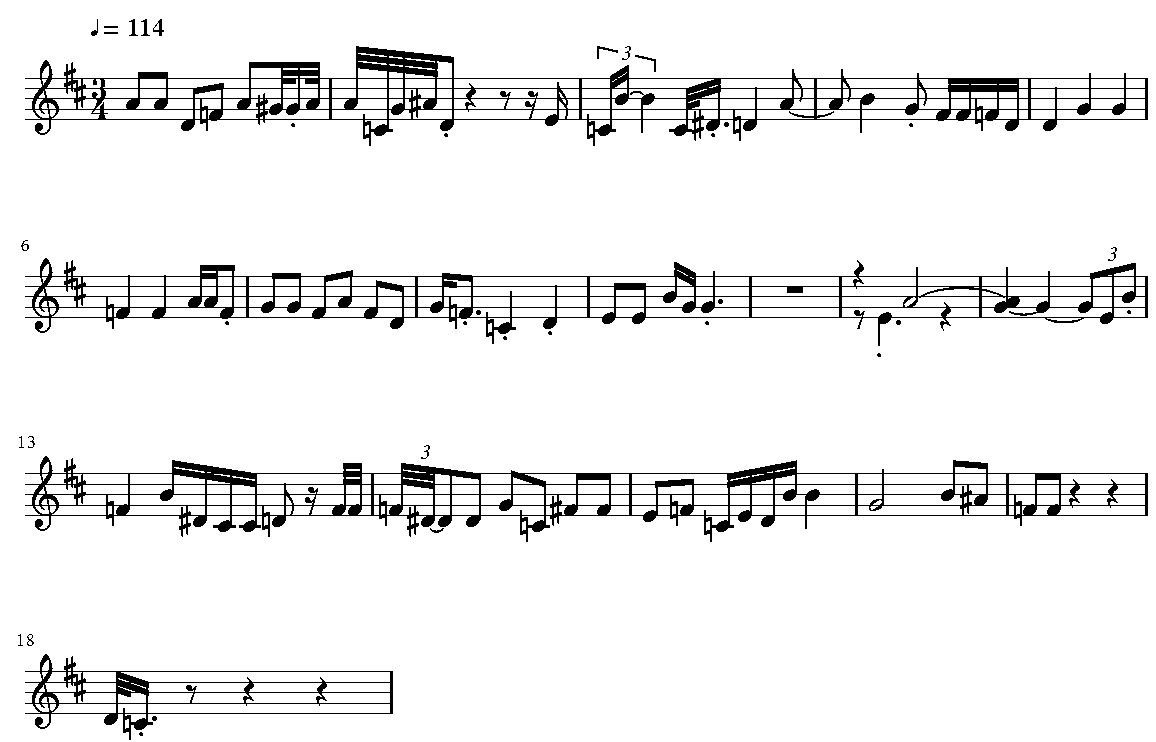
\includegraphics[width=400px]{../images/hmm_melody_generated.pdf}}
\caption{Melody generated with a \ac{HMM}}
\label{ims:hmmmelody}
\end{figure}

Figure \ref{ims:hmmmelody} shows the melody generated with the \ac{HMM}. The resulting melody sounds chaotic and lacks overall structure.


\chapter{Instrumental generation with Markov Chains}
\section{Introduction}
For this experiment a compositional engine will be designed that outputs melodies for a specific instrument. 

In order to construct such an instrumental generator an algorithm is required that can predict time-series data.

A large advantage of recurrent neural networks over Markov chains and \ac{HMM} is that neural networks have greater representational power and can take into account syntactic and semantic features. A \ac{RNN} does not make the Markov assumption and is able to take into account long term dependencies.

Markov chains have the advantage of being much simpler to implement and are extremely fast and efficient with the proper implementation. 
Recurrent Neural Networks are more difficult to implement and to train. Various training algorithms exist to train a \ac{RNN}. Training a recurrent neural network is slower than a regular feed forward network. The poor results obtained from the \ac{LSTM} network (See chapter \ref{ch:accomp_lstm}) dissuade us from using them for the instrumental generator.

This concept will utilize Markov Chains to construct a probabilistic model for a sequence of notes. The probability of the next note occurring depends on the previous state of the chain. See section \ref{sec:markov_backround}.

For a Markov Chain of order $m$ the following holds:
\[
\Pr(X_n=x_n\mid X_{n-1}=x_{n-1}, X_{n-2}=x_{n-2}, \dots , X_1=x_1) =
\\  \Pr(X_n=x_n\mid X_{n-1}=x_{n-1}, X_{n-2}=x_{n-2}, \dots, X_{n-m}=x_{n-m})
\]
For $n > m$

\section{Methodology}
For this technique a different Markov Chain will be constructed for each instrument. 
For a certain instrument, all the notes for that instrument in a MIDI file were added to the Markov chain. This chain is used to generate notes according to a certain instrument.
\begin{algorithm}
 \KwData{MIDI files that accord to a certain style}
 \KwResult{Markov Chain for a particular instrument }
 initialization\;
 \For{each MIDI file}{
  \For{each Instrument}{
    \If{instrument is selected instrument}{
     add notes to Markov chain\;
     }{\;
    }
  }
 }
 \caption{Markov Chain for a particular instrument}
\end{algorithm}

A third order Markov Chain was used. That is, the previous three notes constitute the state of the model. A lower order would result in more novel and random melodies where a higher order would produce melodies with higher similarity.

\section{Results}
\begin{figure}
\centerline{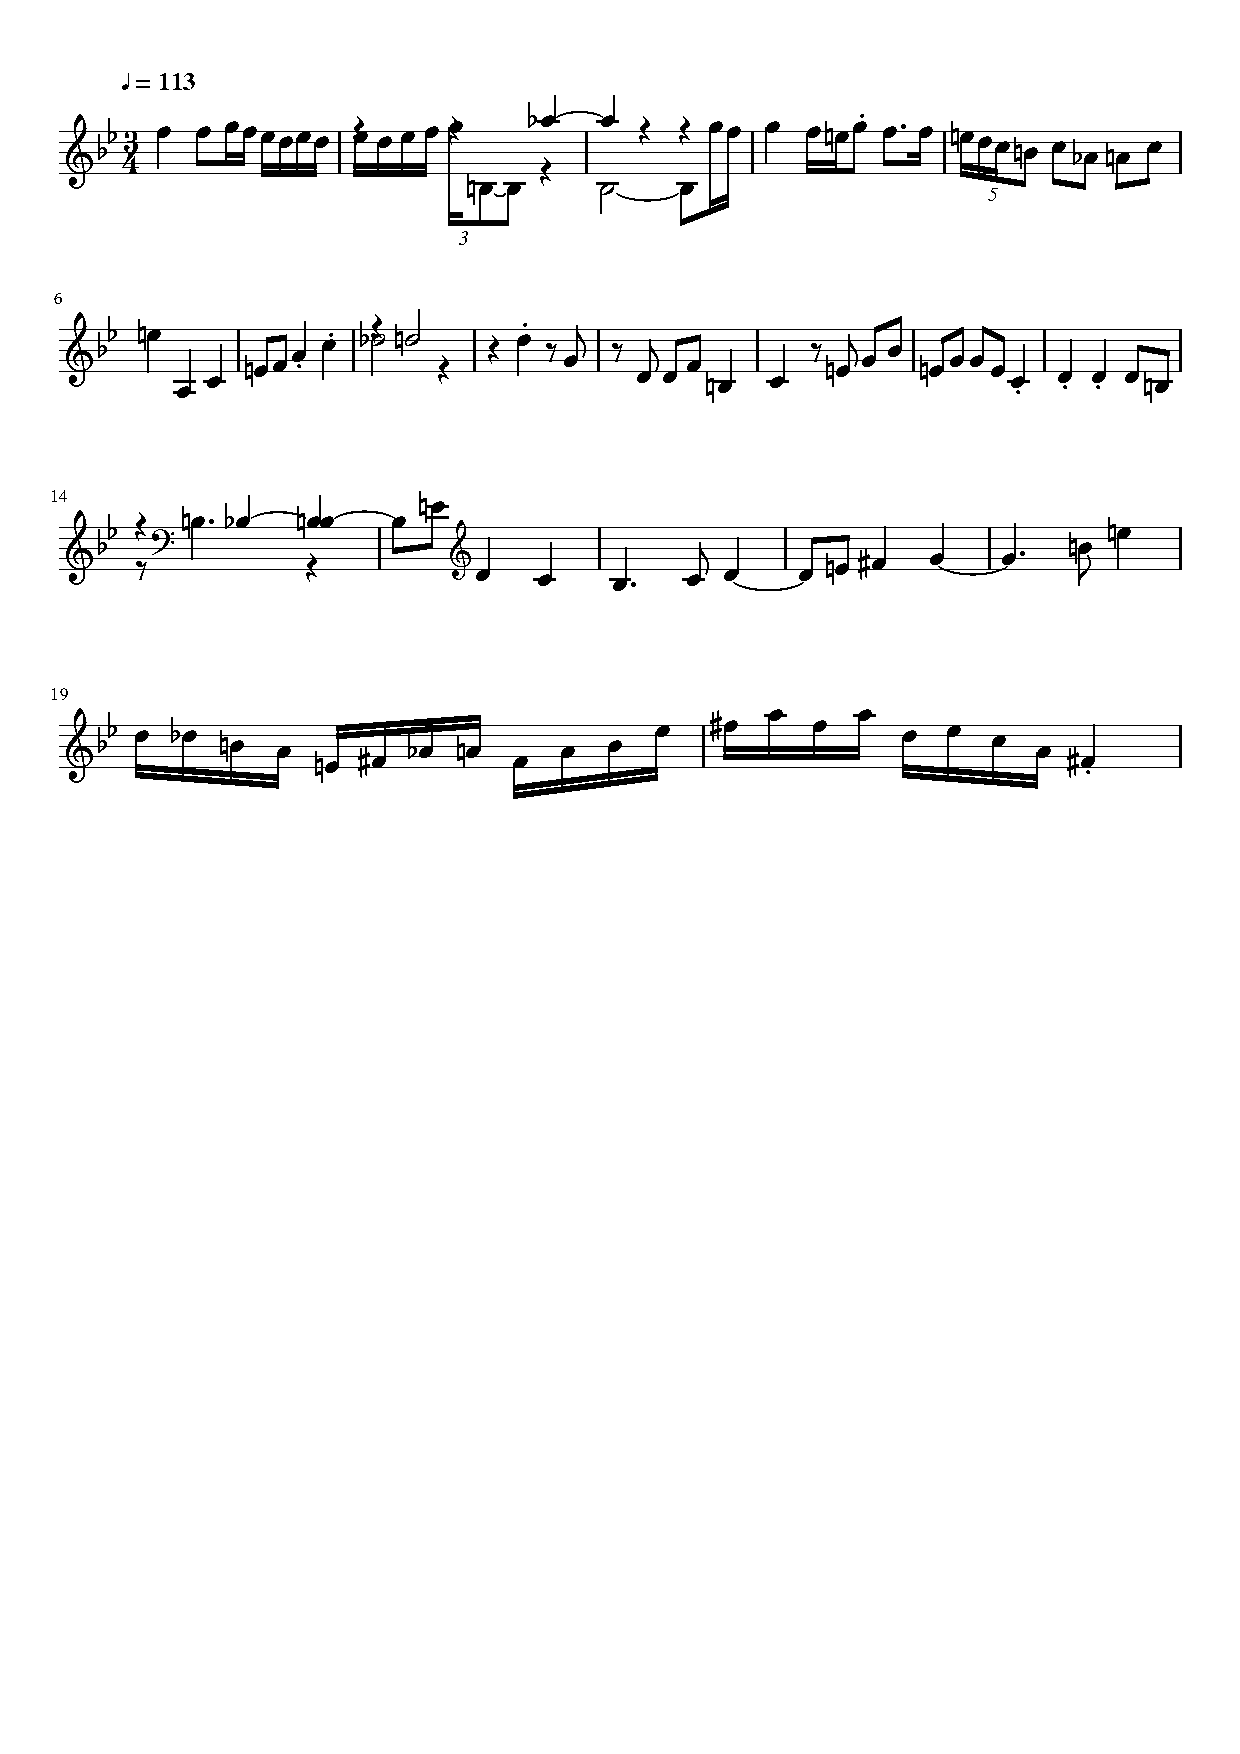
\includegraphics[width=400px]{../images/instrumental_acousticgrand.pdf}}
\caption{Instrumental melody generated with a Markov Chain}
\label{ims:instrumentalmc}
\end{figure}

Figure \ref{ims:instrumentalmc} shows a melody generated with a Markov Chain for the Piano. A third order Markov chain was used with this melody and overall it sounds pleasant. Melodies produced with Markov Chains dont have an overarching theme but do have a local structure and theme.

Melodies produced with Markov Chains are in the same style as the input songs. This reduces compositional value and novelty, especially for higher order Markov Chains. A low order Markov Chain produces more novel although more chaotic and random melodies. 

\section{Potential Improvements}
\begin{itemize}
\item Define which instruments sound good with other instruments
\item Pick which instruments can be slotted together
\item Ensure different tracks accompany each other and are in harmony
\end{itemize}

\chapter{Accompaniment generation with a LSTM network} \label{ch:accomp_lstm}
\section{Introduction}
The \ac{LSTM} network is a \acf{RNN}, however it is more optimized and better suited to classify, process and predict time series in the case when there are long lags of indeterminate length between important events. In this experiment a \ac{LSTM} network is used to generate an accompaniment track for a main melody track

\section{Methodology}
The \ac{LSTM} accompaniment is also generated for a specific instrument. 
Since it is difficult to determine which track is the main melody of a composition an assumption is made that the main melody track is the first track found within a \ac{MIDI} file. The accompaniment track is another track within the \ac{MIDI} file.

For the LSTM network all activation functions were $\tanh$, the network had 2 input units, 15 hidden units, $150$ output units, a learning rate of $0.1$ and momentum of $0.9$.

A list of all possible notes were obtained and the problem was treated as a classification problem. For a set of $n$ possible notes the network has $n$ possible active output units and the active output unit indicates the index of which note was activated. This was done in order to reduce the possibility of incorrect notes as even small error might cause problematic results in alternative representations (if the pitch and duration were used as output).

The input for the neural network is the note pitch and duration of each note in the melody track and the output is the index of the note activated in the accompanied track at the same index.

In order to reduce the dimensionality of the output vector filtering is applied. There are bound to be events that occur rarely which can be seen as noise, and the emphasis should be on more prominent notes.
We apply a simple filtering to discard notes which have a normalized frequency below some threshold in the dataset.
\[ \frac{f}{N} < k \]
where f is the frequency of the note, N the total number of notes and k the threshold.

\begin{algorithm}
 \KwData{MIDI files that accord to a certain style}
 \KwResult{LSTM training for a particular instrument }
 initialization\;
 \For{each MIDI file}{
  \For{each track other than melody track}{
   \If{instrument is selected instrument}{
  \For{each note in melody track and respective note in accompaniment track}{
      add normalized pitch and -duration of current melody note as inputs to dataset\;
      add output note to list of uniques notes\;
      add output note index as normalized output to dataset\;
     }
    }
  }
 }
 
\caption{Training set for LSTM network}
\end{algorithm}
Since a melody track is stored as a sequence of notes, a note in the melody track and a note in the accompaniment track at the same index might not occur at the same time. Thus we iterate through the melody track and use the note closest in time in the accompaniment track for the algorithm.

Training \ac{LSTM} and other recurrent neural networks is slow, as such the weights and structure of the network are saved to storage and is precomputed for each instrument and style of music.

\subsection{Results}
Since the network requires an input melody track to construct an accompaniment track it does not face the same problems such as lack of structure which most other non-recurrent neural networks do.

The output accompaniment can sometimes be pleasant, however a beter timing relation is required between the input and output notes. Most of the produced melodies are repetitive, see figure \ref{ims:lstmaccomp}. The network does not produce an accompaniment which is in harmony or in phase with the main melody track.

\begin{figure}
\centerline{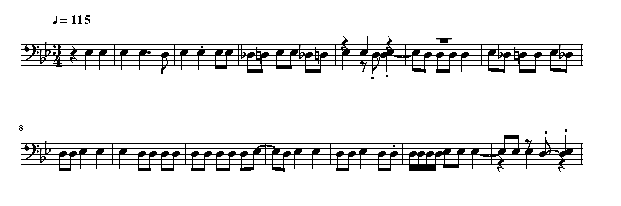
\includegraphics[width=400px]{../images/lstm_accomp.pdf}}
\caption{Accompaniment melody produced with a \ac{LSTM} network}
\label{ims:lstmaccomp}
\end{figure}

The results of the \ac{LSTM} network were surprisingly poor, in comparison with the Markov Chains. A \ac{RNN} has greater representational power and can take into account syntactic and semantic features. A \ac{RNN} also does not make the Markov assumption and is able to take into account long term dependencies. The poor performance of the \ac{LSTM} network is attributed to the implementation and the large training time required for good results.

\chapter{Accompaniment generation with a feed forward network}
\section{Introduction}
In this experiment an attempt is made to generate an accompaniment track for a melody using a feed forward network. One of the reasons for this experiment was to reduce the training time, as recurrent networks have a very large training time.

\section{Methodology}
For this prototype we construct a neural network with the following parameters:
\begin{enumerate}
\item all units use the sigmoid activation function $\frac{1}{e^{-x}}$
\item 1 input layer, 1 hidden layer, 1 output layer
\item 2 input units
\item 2 output units
\item 10 hidden units
\end{enumerate}

The data for the network consists of the melody track and the accompaniment track. For each note in the melody track the note pitch and duration is given as inputs to the network, the output is the note pitch and duration of the corresponding note in the accompaniment track.

\section{Results}
%TODO

\chapter{Accompaniment generation with a Markov Model}
\section{Introduction}
For this experiment an attempt is made to produce an accompaniment based on the frequency of certain notes occuring in the accompaniment track given the melody track.

More specifically, for each note in the melody track the odds are calculated for each possible accompaniment note that may occur at that time. Given an input melody, for each note in that melody an accompaniment note is produced according to the calculated probabilities.

\section{Methodology}
\begin{algorithm}
 \KwData{MIDI files that accord to a certain style\;}
 \KwResult{Accompaniment melody sequence\;}
 \For{each MIDI file}{
  Get main melody\;
  \For{each accompaniment track in file\;}{
    \For{each note $N_m,i$ and previous note $N_{m,{i-1}}$ in main melody and corresponding note $N_a,i$ in accompaniment melody\;}
    {
    	Increment frequency of $N_a,i$ in frequency table for $\{N_m,i, N_m,{i-1} \}$\;
    }
  }
 }
 \caption{Constructing frequency table for model}
\end{algorithm}

\begin{algorithm}
 \KwData{Main melody sequence}
 \KwResult{Accompaniment melody sequence }
 initialization\;
 Create empty accompaniment sequence\;
 \For{each note $N_m,i$ and previous note $N_m,{i-1}$ in main melody sequence}{
  	 Lookup frequencies of possible output notes in frequency table for $\{N_m,i, N_m,{i-1} \}$\;
  	 Obtain probabilities for next notes in frequency table\;
  	 Obtain resulting note according to roulette selection\;
  	 Add resulting note to accompaniment sequence\;
    }
 Return accompaniment sequence\;
 \caption{Obtaining accompaniment melody}
\end{algorithm}


\begin{figure}
\centerline{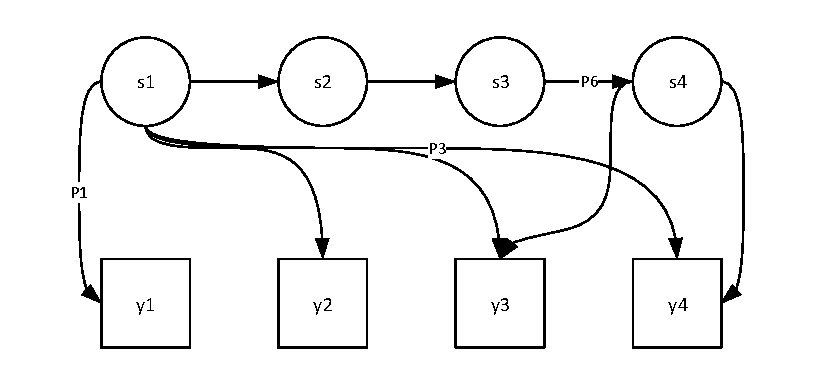
\includegraphics[width=250px]{../images/hmm_illu.pdf}}
\caption{Illustration of a Hidden Markov Model}
\label{ims:hmm_illu}
\end{figure}

Figure \ref{ims:hmm_illu} illustrates a Markov Model. The states $s_i$ denote the notes of the main melody (for a first order Markov Chain) and the states $y_i$ denote the accompaniment notes for melody track. In the case of a \ac{HMM} he states $s_i$ are commonly hidden, however they are known in this case. The states $y_i$ are the output notes that we are interested in generating. 

For this experiment the states are setup up as a second order Markov Chain; that is the next note is determined by the previous two notes. For this model we are not interested in determining thee next state $s_{i+1}$ thus a transmission matrix is not learnt. The probabilities of the output notes $y_i$ are learnt instead.

Since 

\section{Results}
Accompaniment generation with a Markov Model produces better results than with a \ac{LSTM} network. The states of the model are the notes of the main melody and the observations are the notes of the accompaniment. For a short input melody sequence the resulting accompaniment sounds rather pleasant and fits with the main melody. For longer melodies the accompaniment diverges from the main melody and is not in harmony.

\begin{figure}
\centerline{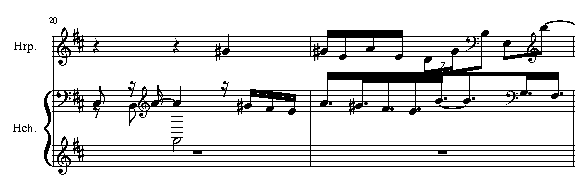
\includegraphics[width=300px]{../images/markov_model_accomp.pdf}}
\caption{Accompaniment generated with Markov Model}
\label{ims:hmm_accomp}
\end{figure}


